\documentclass{beamer} % [aspectratio=169]
\usetheme{ucl}
\setbeamercolor{banner}{bg=brightblue}
\setbeamersize{description width=2em}
\setbeamertemplate{navigation symbols}{\vspace{-2ex}} 

%\usepackage{fontspec}
\usepackage[utf8]{inputenc}
% \usepackage[english, greek]{babel}


\usepackage[T1]{fontenc} % Turn £ into $
\usepackage{minted}
\usemintedstyle{emacs}

\usepackage{fancyvrb}
\usepackage{xcolor}
\usepackage{url}

\usepackage{natbib}
\usepackage{bibentry}
\usepackage{url}


\usepackage{tikz}
\usetikzlibrary{positioning}



\newcommand\emc[1]{\textcolor{brightblue}{\textbf{#1}}}

\AtBeginSection[]{
  \begin{frame}
  \vfill
  \centering
  \begin{beamercolorbox}[sep=8pt,center,shadow=true,rounded=true]{title}
    \usebeamerfont{title}\insertsectionhead\par%
  \end{beamercolorbox}
  \vfill
  \end{frame}
}

\author{Prof.\ George Danezis, University College London, UK}
\title{About ENGS102P.}
\subtitle{ENGS102P: Design and Professional Skills }
% \institute{}
\date{Term 1, 2017}


\begin{document}
\nobibliography*


\frame{
\titlepage
}

\begin{frame}
\frametitle{Notice of Recording \& Questions.}

This course is \emc{video recorded}, and your questions may be recorded too. 
\begin{itemize}
    \item Feel free to not provide your name in questions (I will not).
    \item We intend to make recordings available through moodle and lecture cast.
    \item We intend to upload the recordings to youtube for subtitling.
\end{itemize}

\vspace{3mm}
Please raise your hand at \emc{any time if you have a question}.
\begin{itemize}
    \item Ask for clarifications about the aims of teaching you anything.
    \item Or to help the understanding of the content of the course.
    \item Ask lecturers, and TAs, to speak slowly or write things down to help comprehension.
    \item More will follow \ldots
\end{itemize}

\end{frame} 


\begin{frame}
\frametitle{Welcome to UCL Engineering \& Computer Science!}

Our aim is to prepare you to be the \emc{best engineers in the world}!

\vspace{10mm}
Engineering is the discipline of \emc{shaping the world} around us 

for the \emc{benefit of humanity}.

\vspace{5mm}
\centering

\includegraphics[height=20mm]{img/internet.jpg} \quad
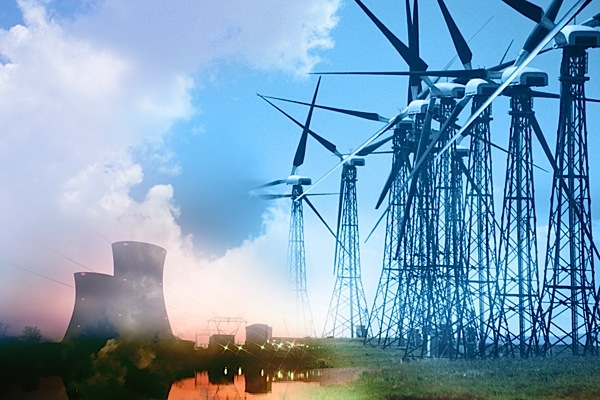
\includegraphics[height=20mm]{img/power.jpg} \quad
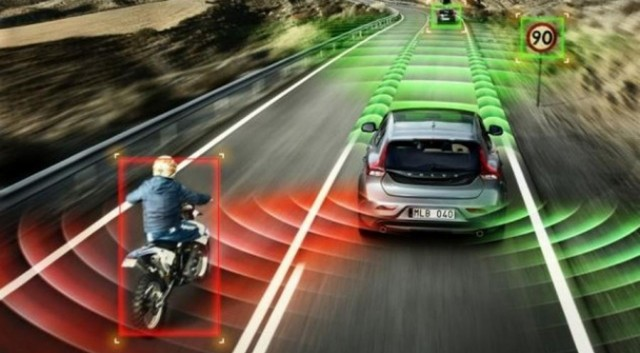
\includegraphics[height=20mm]{img/cars.jpg}

\end{frame}

\begin{frame}
\frametitle{The cost of bad engineering.}

Never forget the \emc{human cost} of bad engineering, 

and your \emc{personal professional responsibility}.

\vspace{10mm}
\centering
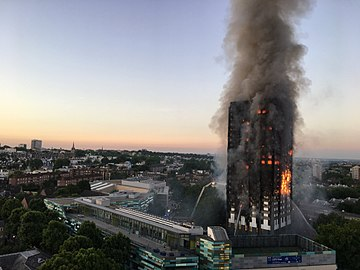
\includegraphics[height=23mm]{img/Grenfell.jpg} \quad
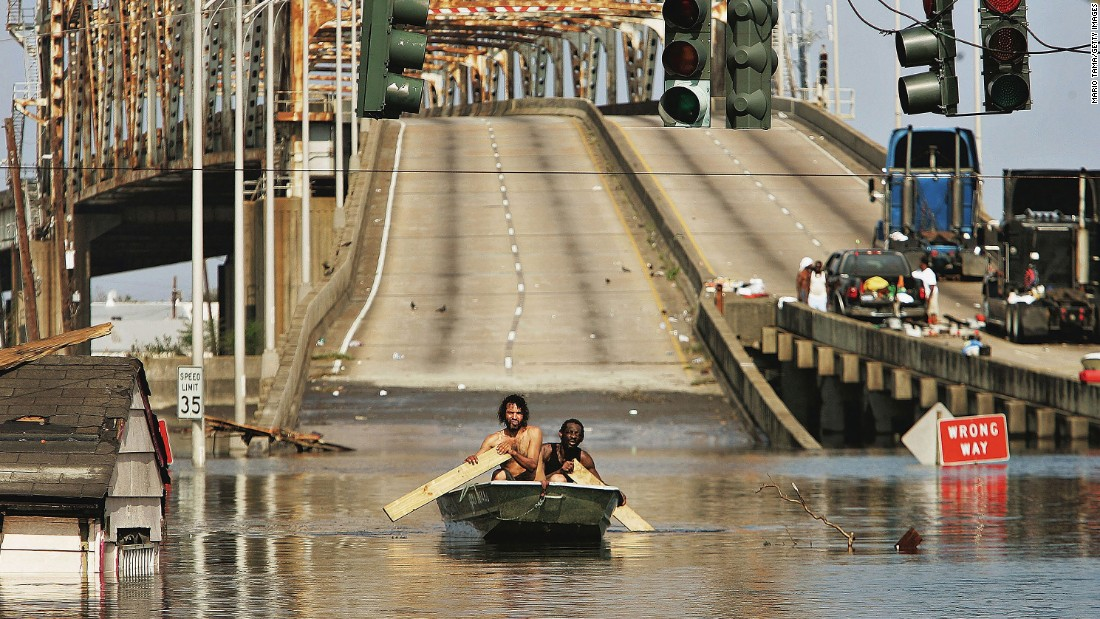
\includegraphics[height=23mm]{img/katrina.jpg} \quad
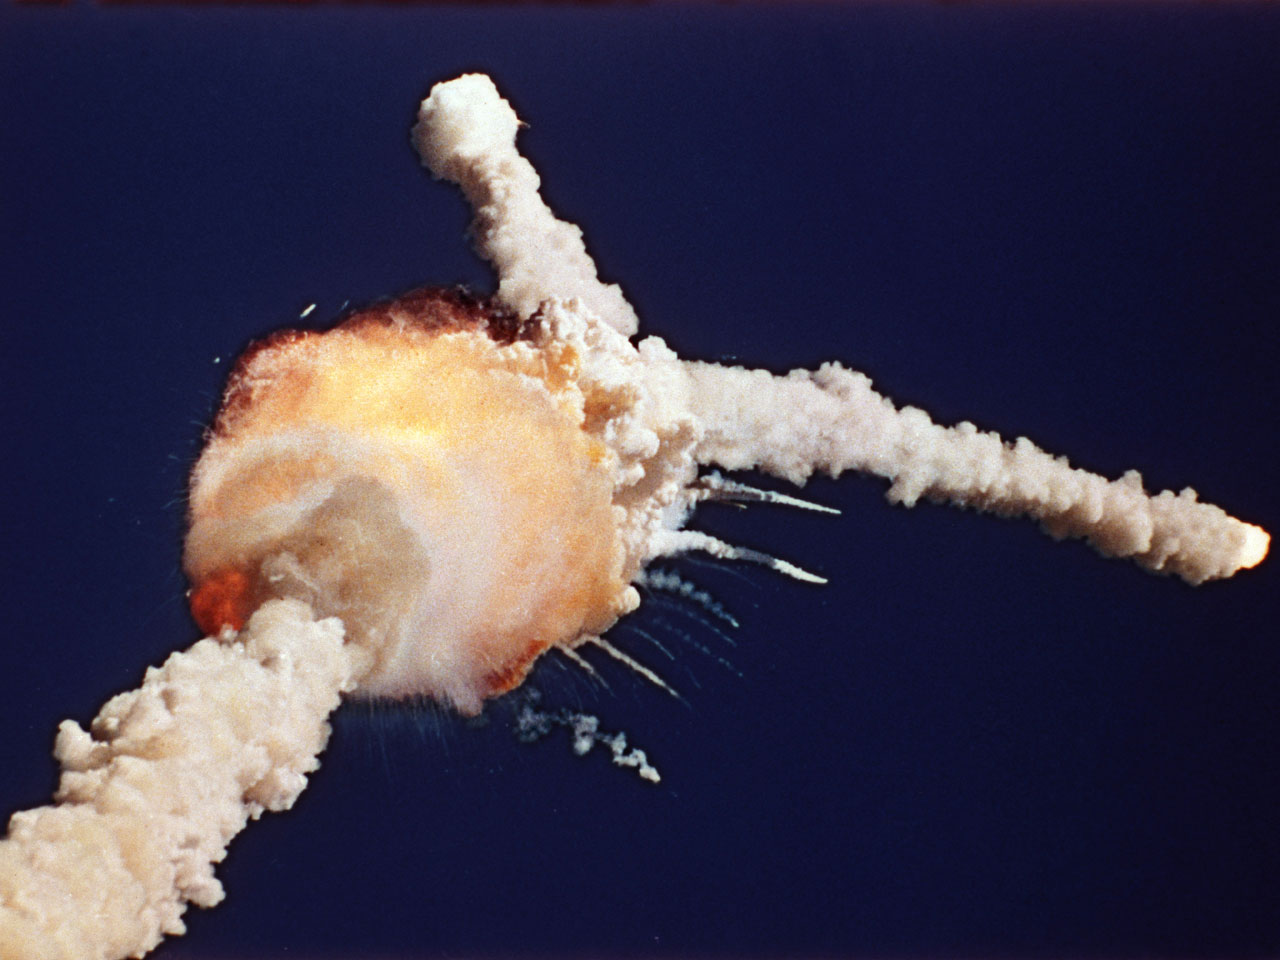
\includegraphics[height=23mm]{img/challenger.jpg}

\end{frame}

\begin{frame}
\frametitle{Overall aims of the ENGS102P.} 

The essence of good engineering is \emc{quality}. This course aims to:

\begin{itemize}
	\item Teach you professional skills important in all engineering.
	\item Teach you computer science specific professional skills.
	\item Expose you to important social and ethical discussions.
	\item Provide opportunities to practice all those skills.
\end{itemize}

\vspace{3mm}
Term 1 teaching is delivered jointly by faculty lecturers and department lecturers. Term 2 is delivered by the department and devoted to software engineering scenarios to support Term 1 concepts.

\end{frame}

\begin{frame}
\frametitle{Who are we? The course leaders.} 

\begin{description}
\item[George Danezis (me)] is a Professor of Security and Privacy Engineering at UCL, with interests in anonymity, privacy, distributed Systems and decentralization.
\item[Stefano Vissicchio] is a Lecturer at UCL, with interests in in theory, algorithms and systems for efficiently and reliably managing communication networks.
\item[Matteo Sammartino] is a Researcher at UCL with interests in formal languages, coalgebras, process calculi, and automata learning.
\item[Kate Roach] is a Senior Teaching Fellow, writer and a researcher with a special interest in the influence of technology, science or engineering on people and vice versa.
\item[Sunny Baines] is a Teaching Fellow, with backgrounds in both technology and journalism, and is a specialist in teaching engineers to communicate.
\end{description}

\end{frame}

\begin{frame}
\frametitle{Who are we? Our teaching assistants.} 

\begin{description}
\item[Alberto Sonnino] is a Ph.D student in Security Engineering with a background in electrical engineering, information technologies and information security.
\item[Leo Joffe] is a PhD student in the Software Systems Engineering group researching the use of information theory and machine learning techniques for software testing and program analysis.
\item[Lisa Chalaguine] is a second-year Intelligent Systems PhD student that is working on chatbot technology for behaviour change, interested in machine learning, human-computer interaction and natural language processing. 
\item[Sam Windels] is a PhD student at UCL with backgrounds in computer science and economics, focusing on network analytics and data integration 
\end{description}

\end{frame}


\begin{frame}
\frametitle{What Engineering Skills?} 

You will spend a significant part of your career \emc{communicating} with other engineers, other professionals and the public.

\vspace{3mm}
To help you we teach:
\begin{itemize}
\item Technical writing \& Technical argument.
\item Engineering visualization.
\item Technical Presentations.
\item Effective team work \& dynamics.
\end{itemize}

\vspace{3mm}
Those are supported with a number of courseworks, feedback \& peer assessment across disciplines.

\end{frame}


\begin{frame}
\frametitle{What Computer Science \& Software Engineering Skills?} 

Computer Science lies at the intersection of \emc{mathematics} and \emc{engineering}. It solves problems through the manipulation of \emc{information}, and \emc{computation}.

\vspace{3mm}
This module will cover:
\begin{itemize}
	\item The \emc{principles of programming} illustrated in Python.
	\item The principles of \emc{algorithms}, their implementation, cost and correctness.
	\item The tools and techniques to ensure \emc{quality software}.
	\item The organization of \emc{software production} in teams.
	\item Key tools and technologies for \emc{rapid prototyping}.
	\item Important \emc{social and ethical} dimensions of the information society.
\end{itemize}

\end{frame}

\begin{frame}
\frametitle{Rough timeline \& Topics.} 

\begin{center}
\begin{tabular}{ c l l }
\hline 
 {\bf Week} & {\bf Tuesday} & {\bf Friday} \\ 
\hline 
W1  & Intro. \& Basics  & \emph{Pebble in the Pond}  \\  
W2  &  Basics & \emph{Visualisation} \\
W3  &  \emph{Technical Argument} & Data Struct. \& Algo.  \\
W4  &  Data Struct. \& Algo. & Dynamic Data Struct. \\
W5  & \emph{Writing} & \emph{Presentation} \\
W6  &  Dynamic Data Struct. & Develop. Practices \\
W7  &  Develop. Practices & \emph{Teamwork} \\
W8  &  Data \& Databases & Data \& Databases \\
W9  &  Networked Apps. & Networked Apps. \\
W10  & Real-world systems & Real-world systems \\
 \hline     
\end{tabular}
\end{center}

\end{frame}

\begin{frame}
\frametitle{Key times, dates and locations} 

The \emc{rooms change every week!}
Familiarize your self with the timetable: \url{https://timetable.ucl.ac.uk}.

\begin{itemize}
	\item Tuesday 09:00--11:00 -- Lectures.
	\item Friday 11:00--13:00 -- Lectures.
\end{itemize}

\vspace{3mm}
Computer Science specific \emc{assessments} due dates \\ (individual programming exercises):
\begin{itemize}
	\item 1 November -- Peer-reviewed exercise.
	\item 29 November -- Assessed exercise.
	\item 10 January -- Assessed exercise.
\end{itemize}
We will provide more information and submission during term.


\end{frame}

\begin{frame}
\frametitle{Pebble in the Pond activity} 

Friday 6 October, 11am-1pm. Jeffery Hall.

\begin{itemize}
	\item You are working in groups of 5-6 (from ENGS101P).
	\item Each group is in charge of a segment of table.
	\item You are provided materials, and need to design a machine.
	\item That takes a pebble (rock) from one end of the set of tables to the other. The pebble must only touch the machine.
	\item Aims: fun, opportunity to meet \& reflections on team work.
\end{itemize}

Arrive promptly at 11am, find your group, and pick a CS table at random quickly! Then listen to the instructions carefully.

\end{frame}

\begin{frame}
\frametitle{Course material.} 

All course material is available on-line, on github and moodle.

\vspace{7mm}
Computer Science specific \emc{syllabus, slides \& code}: 

\url{https://github.com/gdanezis/Design_and_Professional_Skills}

\vspace{7mm}
To support you while learning the Python programming language:

\vspace{2mm}
Allen Downey. \emc{Think Python}. Green Tea Press. (free e-book)

{\small \url{http://greenteapress.com/thinkpython/thinkpython.pdf} }

\vspace{2mm}
Bruce Eckel. \emc{Thinking in Python}. (More advanced)

{\small \url{http://docs.linuxtone.org/ebooks/Python/Thinking_In_Python.pdf} }


\end{frame}

\begin{frame}
\frametitle{How to seek help with the course.} 

Use the Moodle discussion board first for questions: 
\url{https://moodle.ucl.ac.uk/course/view.php?id=43301&section=15}

\vspace{3mm}
Our excellent team of TAs help with questions and provide feedback:
\begin{itemize}
\item Alberto Sonnino --- \url{alberto.sonnino@cs.ucl.ac.uk}
\item Leonid Joffe --- \url{leonid.joffe.14@ucl.ac.uk}
\item Lisa Chalaguine --- \url{lisa.chalaguine.16@ucl.ac.uk}
\item Sam Windels --- \url{sam.windels.16@ucl.ac.uk}
\end{itemize}

\vspace{3mm}
Office hours of course leaders:
\begin{itemize}
\item George Danezis --- Tuesday 11:00--13:00 MPEB 4.13
\item Stefano Vissicchio --- Wednesday 11:00--12:00 MPEB 6.17
\item Matteo Sammartino --- 
\end{itemize}

\end{frame}

\begin{frame}
\frametitle{How to communicate issues about the course.}

We always welcome your feedback to improve courses!

\vspace{3mm}
Provide feedback and fixes to course material using the Github issue tracker:
\url{https://github.com/gdanezis/Design_and_Professional_Skills/issues}

\vspace{3mm}
You are welcome to bring up any issues to:
\begin{itemize}
	\item the \emc{course leaders or TAs}.
	\item the \emc{1st year coordinator} (\url{J.Brotherston@ucl.ac.uk}).
	\item our Dept. \emc{teaching team} (\url{n.gosai@ucl.ac.uk}).
	\item the \emc{Director of Studies} (\url{A.Silva@cs.ucl.ac.uk}).
	\item the \emc{Head of Department} (\url{J.Shawe-Taylor@cs.ucl.ac.uk})
\end{itemize}

\end{frame}

\begin{frame}
\frametitle{Professionalism \& Code of Conduct (I).}

We expect you to keep a very high standard of \emc{professionalism} in this course. Including a high degree of \emc{courtesy} in all your interactions, and \emc{integrity} when it comes to assessment.

\vspace{3mm}
The \emc{British Computing Society} (BCS) defines a code of conduct:
\begin{description}
	\item[The Public interest]: Respect for public health, privacy, security and wellbeing of others and the environment. Respect the rights of others. Conduct activities without discrimination, and extend to all the benefits of computing.
	\item[Competence and Integrity]: do not overclaim your competence, and only accept work within it; keep up professional development; respect all view points and offer honest opinions; do not be malicious or neglectful; do not bride or be bribed.
\end{description}

\end{frame}

\begin{frame}
\frametitle{Professionalism \& Code of Conduct (II).}

\begin{description}
	\item[Duty to Relevant Authority]: Implement diligently requirements, while exercising your judgment; avoid conflicts of interest; accept personal responsibility for your work and reports; keep confidences; and do not withhold relevant information.
	\item[Duty to the profession]: improve standards in the profession; support the BCS activities and members, and do not bring it into disrepute.
\end{description}

\vspace{3mm}
Full code of conduct: \url{http://www.bcs.org/category/6030}.

\vspace{3mm}
If ever in doubt please approach us for discussion or advice.

\end{frame}


% ---------------------------------

\bibliographystyle{alpha}
\nobibliography{references}

\end{document}